\section{Fiducial Mass and Volume}
\label{sec:fidmassvol}

To calculate the $\nu_\mu$ inclusive charged current cross section, proper evaluation of the number of target nucleons is of paramount importance. This requires a clear description of an analysis fiducial volume and the measurement of the mass contained in said volume. The determination of the fiducial volume was made based on the design of the detector and the requirements of analyses predominantly concerned with selecting electromagnetic showers. Table \ref{tab:FV} lists the fiducial volume boundaries used in most analyses using the P0D. They are chosen to minimize the uncertainty on the water mass enclosed in the water target and are placed around 25~mm from the X and Y edges of the detector. These boundary values as well as all future coordinates are given with respect to the ND280 coordinate system shown in Figure \ref{fig:nd280geom}. The Z direction boundaries are chosen to primarily enclose all the water layers in the P0D. More specifically, they are placed between the X and Y layers of the two p0dules that bound the upstream and downstream ends of the water target. Since there are lead radiators in the ECALs that sandwich the water target and the interaction rates on lead are not well known, this Z axis range allows us to reject unwanted lead events while efficienctly selecting water events. 

\begin{table}[h]
\caption{The P0D Water-Target Fiducial Volume boundaries given in the ND280 coordinate system. All units are in mm.}
\centering
\begin{tabular}{ccc}
\toprule
Axis & FV (min) & FV (max) \\
\hline
X & -836 & 764 \\
Y & -871 & 869 \\
Z & -2969 & -1264 \\
\bottomrule
\end{tabular} 
\label{tab:FV} 
\end{table}

The fiducial mass of the non-water components of the P0D was determined from careful measurements during the construction of the detector. This work was completed by a few group members to provide a baseline for all P0D based analyses. We summarize the procedure and results from their work. The measurements are made for four separate elements of the P0D: brass radiators, upstream water target cover, p0dules and water. The thickness of the brass radiator sheets was measured prior to assembly and the standard density of brass used to calculate the mass. Water target covers are present to provide structural support to the outer water bag layers and are made of high-density polyethylene (HDPE). The thickness of these covers was provided by the manufacturer and the density was averaged from an online list of HDPE densities.

Each p0dule is constructed from two light-tight covers, two scintillator planes, 260 wavelength-shifting (WLS) fibers and three layers of epoxy to hold it all together. The mass of the light-tight covers was calculated by measuring their thickness and using an online list of density. The mass of each scintillator plane was measured during construction and the areal density was calculated using the total mass and fiducial area. The design thickness of each epoxy layer was used in conjunction with the known density of epoxy to calculate the mass of the three epoxy layers. Finally, the mass of the WLS fibers was calculated from the diameter and density extracted from the design specifications. The WLS fibers cross the entire height and width of the fiducial volume so the X and Y ranges were used for the fiber length. The errors on the non-water fiducial mass stem primarily from the thickness measurements and the scale used to weigh the P0Dules. They are combined by treating each component mass error as independent.

The MC fiducial mass does not use any of these specific measurements directly. Instead, the ND280 simulation geometry is density averaged and this average is multiplied by the fiducial volume. Table \ref{tab:aden} summarizes the areal density of the three non-water components of the P0D. It is important to note here that our analysis ideally subtracts out the event rate from non-water elements of the P0D. The target number in the cross section formula does not depend on the non-water fiducial mass whatsoever. This information is stated primarily for completeness.

\begin{table}[h]
\caption{The areal density of three of the four major elements of the P0D in the fiducial volume. All units are in gm/cm$^2$.}
\centering
\begin{tabular}{ccc}
\toprule
Material & Data Areal & MC Areal\\
& Density (g/cm$^2$) & Density (g/cm$^2$) \\
\midrule
Brass & $1.088 \pm 0.032$ & 1.09 \\
WT Cover & $0.024 \pm 0.002$ & 0.02 \\
P0Dule & $3.843 \pm 0.034$ & 3.84 \\
\bottomrule
\end{tabular} 
\label{tab:aden} 
\end{table}

The final component of the P0D in the fiducial volume is water. As this is our cross section target, this is also the most crucial measurement. All measurement errors translate directly to uncertainties on the cross section, so the treatment of systematics is also very important. To fill the P0D, water is pumped from a main holding tank through fill pipes and into the water bags located in the water target. The external water tank is equipped with a depth sensor and a sight glass mounted to monitor the water level inside. To measure the amount of water in the fiducial volume of the water target, the sight glass is used to observe the change in water level over the fill period and the height change is converted to water mass. This water mass is then corrected for any losses during the fill procedure and scaled down to the fiducial volume. The fiducial mass of the water ($M_{fid}$) is given by:
\begin{equation*}
M_{fid} = (C_{dm}\times H_{fid} - M_{drip} - M_{config} - M_{overshoot}) \times R_{x~cut}
\end{equation*}

Here, $C_{dm}$ is a factor that converts water level change in the main tank to water mass and $H_{fid}$ is the height change of the water in the tank over the fill period. The terms $M_{drip}$, $M_{config}$ and $M_{overshoot}$ are corrections for losses of water while filling, configuration changes in the water system and overfilling the fiducial volume respectively. To determine $C_{dm}$, 80~L buckets of water were filled from the main tank while using the sight glass to record the change in water level from each bucket fill. The water mass in the bucket was measured using a 100~kg digital scale calibrated with precision, $20$~kg$\pm 1$~g weights. The measured masses of the water buckets were plotted against the change in height of the water level. Some of the data points were rejected due to depth sensor readings that were inconsistent with the height change. The multiplicative height to mass conversion term $C_{dm}$ is the mean of the remaining data points. From two calibration runs, the $C_{dm}$ vaue is $1.0696 \pm 0.0077$~kg/mm. The data from one such calibration run is shown in Figure \ref{fig:cdm}. The sources of error on $C_{dm}$ are a $5\%$ instrument error from the weighing scale and a 2~mm uncertainty from the sight glass.

\begin{figure}
\centering
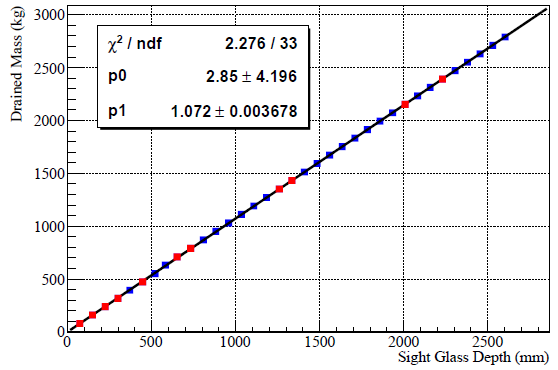
\includegraphics[width=3.2in]{Figures/cdmline.png}
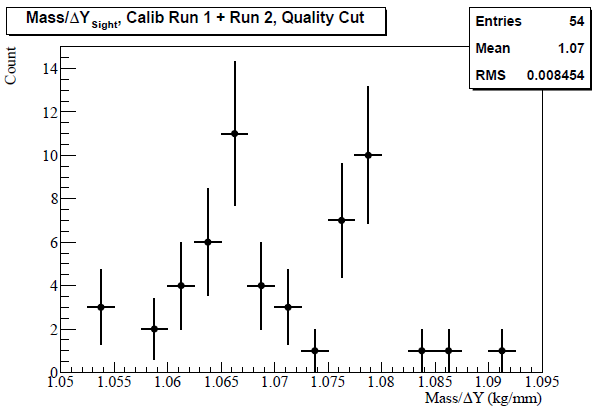
\includegraphics[width=3.2in]{Figures/cdmhist.png}
\caption{Left: Measured water mass in each bucket vs. sight glass depth reading for the first of two calibration runs. The red points were rejected due to inconsistency between sight glass and main tank depth sensor readings. Right: A histogram of the ratio of measured water mass and the change in water depth after the faulty data points were removed. The mean of the remaining data points is used as the $C_{dm}$ value.}
\label{fig:cdm}
\end{figure}

Calibration fill runs were performed to evaluate the water level change ($H_{fid}$) expected when filling the fiducial volume with water. Each water bag in the P0D is equipped with a depth sensor. The bags were systematically filled a little at a time until the average depth readings over all bags equaled the lower fiducial Y boundary. The location of the water level in the main tank was marked. Similarly, the bags were filled to the upper Y boundary of the fiducial volume and another mark was placed on the main tank. The distance between these two marks is used for the water level height change $H_{fid}$. 

There are three corrections to the initial water fiducial mass calculation. The first correction, $M_{drip}$ accounts for water lost from dripping or spillage during the filling process. The total amount is very small and is estimated conservatively by eye to be $4\pm1$~kg. The second correction comes from a change in the water system configuration made after the initial main tank calibrations. An updated pumping system causes a loss in the amount of water delivered to the water bags from the main tank. This loss, $M_{config}$ is estimated to be $10\pm2$~kg. The final correction attempts to adjust for an inaccuracy in the main tank fiducial volume fill marks. The two marks on the main tank were placed by filling water bags until the \emph{average} water level in each bag was at the fiducial volume boundaries. However, it is nearly physically impossible to fill the bags to exactly where the fiducial boundaries are, so in reality the average was around 1.5~cm above the Y fiducial boundary. The correction was calculated by adding together the individual bag depth readings and comparing this to the nominal cumulative depth expected from the fiducial volume. Overfilling the bags by 1.5~cm on average corresponds to a difference of $823\pm48$~mm of water, which is $23\pm2$~kg of water. This is the value used for the $H_{overshoot}$ correction term. 

The final term in the fiducial mass equation is a multiplicative factor $R_{x~cut}$ that scales the fiducial mass down to account for the X directional boundaries. There is a vertical supportive strut in the middle of each water bag layer that separates the two water bags in each layer. Removing the width of this strut, the total width in the X direction of the water bags is $1995\pm5$~mm and the width of the fiducial volume is $1585\pm5$~mm. The ratio of the two widths is $0.794\pm0.003$ and is used as the value of $R_{x~cut}$. All the errors are treated as independent, so the final water fiducial mass with errors added in quadrature is:

\begin{equation}
M_{fid} = 1902 \pm 16 (0.8\%)~kg
\end{equation}

Now we are able to calculate the total number of target nucleons for the cross section formula. A simple calculation using Avogadro's constant and the molar mass of water yields $T_w$, the total number of nucleons in the water fiducial mass.
\begin{equation}
\label{eqn:tarnum}
T_w = \frac{6.022141\times10^{23}}{\text{mol}}\times \frac{\text{mol}}{18.015~g} \times \frac{18~\text{nucleons}}{H_2 O molecule} \times 1902~\text{kg} = 1.145 \times 10^{30} \text{nucleons}
\end{equation}
